\documentclass[sigconf]{acmart}
\usepackage{tikz}
\usetikzlibrary{shapes.geometric}
\usetikzlibrary{matrix}
\usepackage{environ}
%%
%% \BibTeX command to typeset BibTeX logo in the docs
\AtBeginDocument{%
  \providecommand\BibTeX{{%
    Bib\TeX}}}

\setcopyright{acmlicensed}
\copyrightyear{2025}
\acmYear{2025}
\acmDOI{XXXXXXX.XXXXXXX}
%% These commands are for a PROCEEDINGS abstract or paper.
\acmConference[FPGA '26]{International Symposium on Field Programable Gate Arrays}{June 03--05,
  2025}{Seaside, CA}
%%
%%  Uncomment \acmBooktitle if the title of the proceedings is different
%%  from ``Proceedings of ...''!
%%
%%\acmBooktitle{Woodstock '18: ACM Symposium on Neural Gaze Detection,
%%  June 03--05, 2018, Woodstock, NY}
\acmISBN{978-1-4503-XXXX-X/2018/06}

\begin{document}

\title{Yet Another Multi-Port Memory for FPGAs}

%%
%% The "author" command and its associated commands are used to define
%% the authors and their affiliations.
%% Of note is the shared affiliation of the first two authors, and the
%% "authornote" and "authornotemark" commands
%% used to denote shared contribution to the research.
\author{Kevin Townsend}
\email{kt@krtownsend.com}

\renewcommand{\shortauthors}{Townsend et al.}

\begin{abstract}
  We propose a simple extention to XOR memories presented in previous work.
In this paper we generalize the XOR memory. We explore the resource usage on Xilinx/AMD
FPGAs.
\end{abstract}

%%
%% The code below is generated by the tool at http://dl.acm.org/ccs.cfm.
%% Please copy and paste the code instead of the example below.
%%
%\begin{CCSXML}
%<ccs2012>
% <concept>
%  <concept_id>00000000.0000000.0000000</concept_id>
%  <concept_desc>Do Not Use This Code, Generate the Correct Terms for Your Paper</concept_desc>
%  <concept_significance>500</concept_significance>
% </concept>
% <concept>
%  <concept_id>00000000.00000000.00000000</concept_id>
%  <concept_desc>Do Not Use This Code, Generate the Correct Terms for Your Paper</concept_desc>
%  <concept_significance>300</concept_significance>
% </concept>
% <concept>
%  <concept_id>00000000.00000000.00000000</concept_id>
%  <concept_desc>Do Not Use This Code, Generate the Correct Terms for Your Paper</concept_desc>
%  <concept_significance>100</concept_significance>
% </concept>
% <concept>
%  <concept_id>00000000.00000000.00000000</concept_id>
%  <concept_desc>Do Not Use This Code, Generate the Correct Terms for Your Paper</concept_desc>
%  <concept_significance>100</concept_significance>
% </concept>
%</ccs2012>
%\end{CCSXML}
%
%\ccsdesc[500]{Do Not Use This Code~Generate the Correct Terms for Your Paper}
%\ccsdesc[300]{Do Not Use This Code~Generate the Correct Terms for Your Paper}
%\ccsdesc{Do Not Use This Code~Generate the Correct Terms for Your Paper}
%\ccsdesc[100]{Do Not Use This Code~Generate the Correct Terms for Your Paper}

%%
%% Keywords. The author(s) should pick words that accurately describe
%% the work being presented. Separate the keywords with commas.
%\keywords{Do, Not, Us, This, Code, Put, the, Correct, Terms, for,
%  Your, Paper}
%% A "teaser" image appears between the author and affiliation
%% information and the body of the document, and typically spans the
%% page.
\begin{teaserfigure}
  %\includegraphics[width=\textwidth]{sampleteaser}
  \begin{center}
  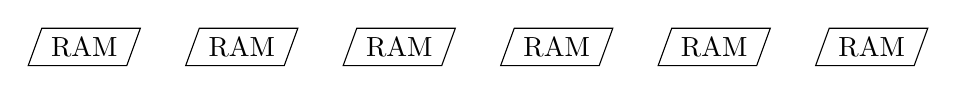
\begin{tikzpicture}[scale=2]
  \foreach \x in {0,1,2,3,4,5} {
    \node [trapezium, trapezium left angle=70, trapezium right angle=110, draw] at (\x, 0){RAM};
  }
  %TODO: draw 2d array of nodes.
  %TODO: draw xor of read ports
  %TODO: draw ports
  %TODO: draw xor of write ports
  %TODO: draw xor of full ports
  \end{tikzpicture}
  \end{center}
  \caption{Seattle Mariners at Spring Training, 2010.}
  \Description{Enjoying the baseball game from the third-base
  seats. Ichiro Suzuki preparing to bat.}
  \label{fig:teaser}
\end{teaserfigure}

\received{20 February 2007}
\received[revised]{12 March 2009}
\received[accepted]{5 June 2009}

%%
%% This command processes the author and affiliation and title
%% information and builds the first part of the formatted document.
\maketitle

\section{Motivation}

As computation needs keep increasing with Moore's Law one way to keep up has been
specialized architectures. FPGAs provide a way to implement architectures without taping out an ASIC.
However, the limitations of FPGA resources means some creativity is needed to map designs to FPGAs.
This paper explores the limitation of FPGAs in the fact that FPGA memories have a limited number of
ports. Specifically we look at creating memories with more than 2 ports.

The 3 major FPGA vendors implement distributed memory (small memories) and block memory (large memories)
differently, however they share some characteristics.

All 3 vendors support distributed memory configurations with 1 full port and up to 3 read ports.

All 3 vendors support block memory with 2 full ports.

\section{Source Code}
We provide all of the source code used in implementation and testing our design at
github.com/kevintownsend/mpm. We tested our design with Verilator and implemented the design
with Vivado (Xilinx/AMD).

\section{Introduction}

We propose a simple generalization to XOR memories presented in previous work.
XOR memories work by using the a xor b xor b = a property. We add bidirectional
ports and analyze the perforamance of distributed memory and block memory
versions of this design. We also present applications for these memories.

We also present a LVT memory that utizazes distrubuted memory xor live value table.

\section{Live Value Table Memory}

In (TODO citation) the live value table was implemented with registers. Previous work used
distributed memory (TODO citation). However they did not use bidirectional xor ports in their implementation.

We create a LVT memory using the technique described in (TODO cititaion). TODO: describe technique.

We show we utilize x\% less resources than LVT and I-LVT.

\section{Impractical Designs}

We obviously wanted to explore impractical designs with large numbers of ports. We say
impractical because of the high resource usage of XOR and LVT memories at high port counts.
N**2 for XOR and N*(N-1)/2 for LVT. However we were able to synthesize a 16 port memory.

Without write delay the design runs at Xmhz (x\% of max). With write delay and pipelining the design runs at Xmhz.

\section{Conclusion}
Several solutions to the port limit on FPGAs other than what is presented here.
For example multi-pumping and banking. multi-pumping is the process of reducing
the clock speed to increase the number of ports. For example a 300Mhz single
port memory can handle 2 150Mhz ports. Banking requires stalls and routing logic
due to the segmented memory. Our design uses replication and some creativity
XOR and LVT to create multiple ports.

%% The next two lines define the bibliography style to be used, and
%% the bibliography file.
\bibliographystyle{ACM-Reference-Format}
\bibliography{sample-base}


%%
%% If your work has an appendix, this is the place to put it.
%\appendix

\end{document}
\endinput
%%
%% End of file `sample-sigconf.tex'.
